\chapter{Topic Modelling}\label{ch:topic-modelling}
\section{Information Extraction Types}

Information Extraction in \gls{nlp} can be subdivided into multiple fields \cite{iebook}, among them:

\begin{itemize}
    \item \textbf{Relation Extraction}: Extraction and classification of relations between named entities
    \item \textbf{Event Extraction}: Extraction of a temporal Event
    \item \textbf{Topic Modelling}: Assigment of a topic to a short text or document
\end{itemize}

The initial expectation for this project was to extract information from the article sentences in the form of triples:

\begin{center}
\textbf{Triple: Subject – Relation – Object}
\end{center}

where either the Subject or the Object would be a corporate entity (\gls{org}).

If the Subject were a company, the Object could either be another company or any other common named entity type from the set of \gls{org}, \gls{per} or \gls{loc}, and vice versa.

The assumption was that these Subjects and Objects would appear in the same sentence as in the following example:
\begin{figure}[H]
    \centering
    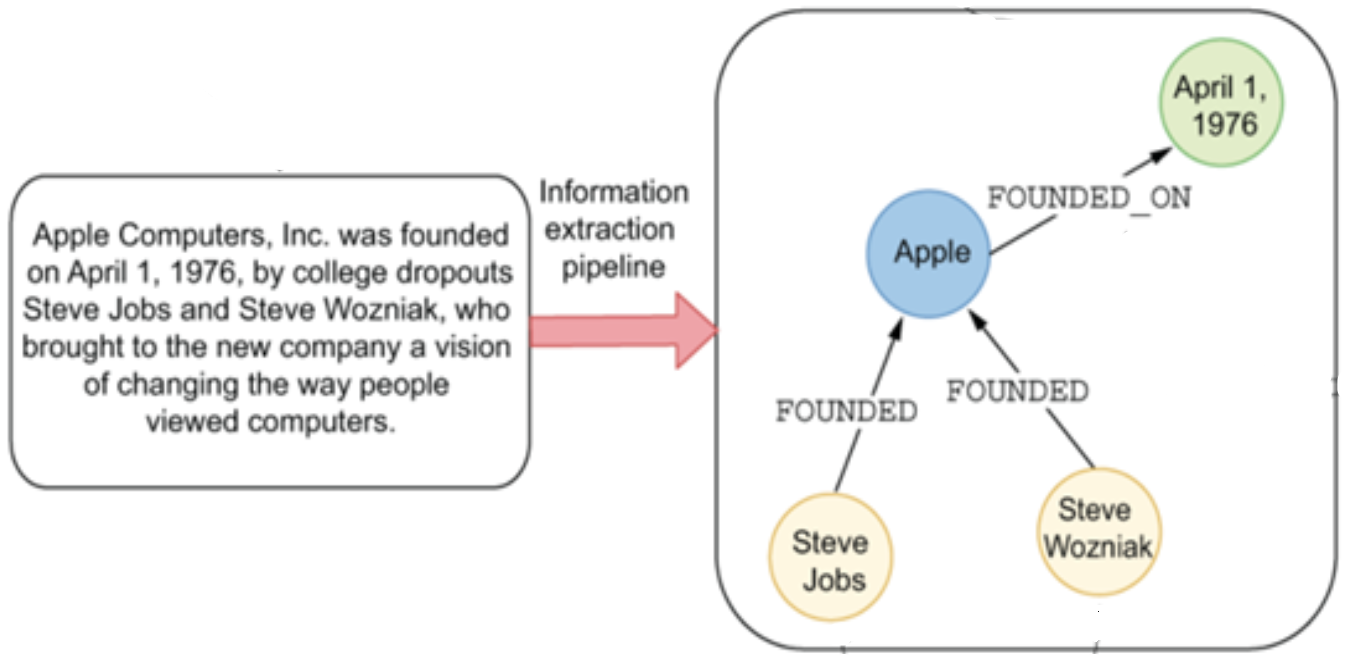
\includegraphics[width=1.0\textwidth]{Assets/sub-pred-obj}
    \caption{Triple: Subject: Person - Relation: Founded - Object: Apple}
    \label{fig:triples}
\end{figure}

After investigation of the news articles, it became clear that the limitation to only extract Relation triples was too restrictive.
Many article sentences only contained one common named entity type or described an Event rather than a relationship between entities.

In some other sentences, Subjects or Objects could have been assigned to a wider and less common set of entity types such as \emph{Product}, \emph{Money} or \emph{Law},
but this would have required to enlarge the set with many new custom entity types to cover the most fundamental themes in the finance domain.

It would also have meant to increase the complexity of the Knowledge Graph and deviate from the goal of the project, which was
to extract information from news articles with a focus on particular companies.
To answer the central question
\begin{center}
    \textbf{What is the company news all about?}
\end{center}
a more general and more comprehensive extraction type was needed.


Topic Modelling can be done on the sentence level and does not require entity pairs.
Topics can cover Events as well as Relations between entities and a wide array of finance themes.
Extracting information via Topic Modelling thus seems more appropriate for the data and task given than Relation Extraction.

\section{Traditional Topic Modelling}\label{sec:traditional_approaches}
Most of the traditional Topic Modelling methods are based on absolute (Bag-of-Word: Section \ref{subsec:bag-of-words}) or relative (TF-IDF: Section \ref{subsec:tf-idf}) word counts as discussed in Section \ref{ch:text-representation}.

They also return topics in the form of most frequent words where the user must first read the words per topic to get a sense of what the topic is all about, see Figure \ref{fig:lda-out}.

\begin{figure}[H]   %[h] puts picture right here. 't' stands for to, 'b' stands for bottom
    \centering
    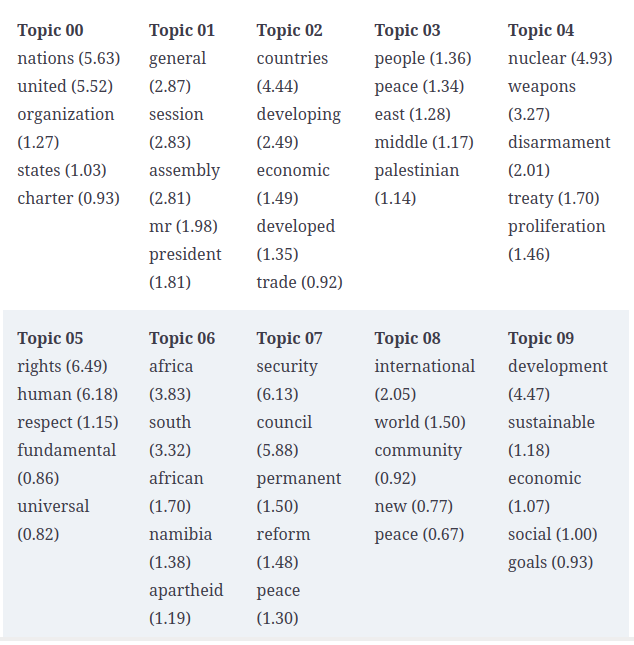
\includegraphics[width=0.60\textwidth]{Assets/lda-out}
    \caption{10 Topics and their most frequent words. Source: \cite{blueprints}}
    \label{fig:lda-out}
\end{figure}

\subsection{\gls{nmf}}\label{subsec:nmf}
In the Non-Negative Matrix Factorization method (\gls{nmf}), the most frequent words are retrieved by doing a
matrix decomposition of the \gls{document_term_matrix} (see Section \ref{fig:document_term_matrix}) which in the following Figure is dubbed \emph{Documents-Words Matrix}:

\begin{figure}[H]   %[h] puts picture right here. 't' stands for to, 'b' stands for bottom
    \centering
    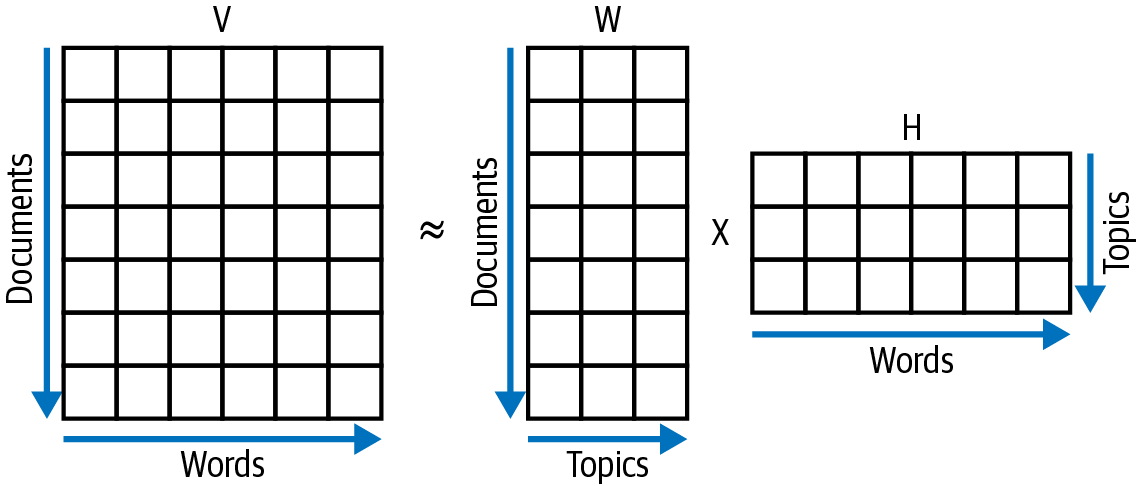
\includegraphics[width=0.70\textwidth]{Assets/nmf}
    \caption{\gls{nmf}: Source: \cite{blueprints}}
    \label{fig:nmf}
\end{figure}

The Documents-Topics matrix in the middle of Figure \ref{fig:nmf} maps Documents to Topics whereas the Words-Topics matrix on the right maps topics to their features, i.e. the words in the \gls{vocabulary}.
In most implementations, a rank parameter (or \emph{n\_components} parameter in Scikit-Learn's implementation \cite{nmf-implementation}) can be provided so that the word dimension of the \gls{document_term_matrix} first gets reduced before it is decomposed.
Because of this, \gls{nmf} can also be used as a dimension reduction method \cite{nmf-implementation}.
To get the most frequent words, each row in the Words-Topics matrix is sorted by its highest values with their respective column indexes being looked up in the \gls{vocabulary}.
The number of topics can be chosen arbitrarily but a smaller number will "throw" more words into one topic which makes the decomposition less exact \cite{blueprints}.

\subsection{\gls{svd}}\label{subsec:svd}
A very similar method is the Singular Value Decomposition (\gls{svd}) that decomposes the \gls{document_term_matrix} into three matrices:

\begin{figure}[H]   %[h] puts picture right here. 't' stands for to, 'b' stands for bottom
    \centering
    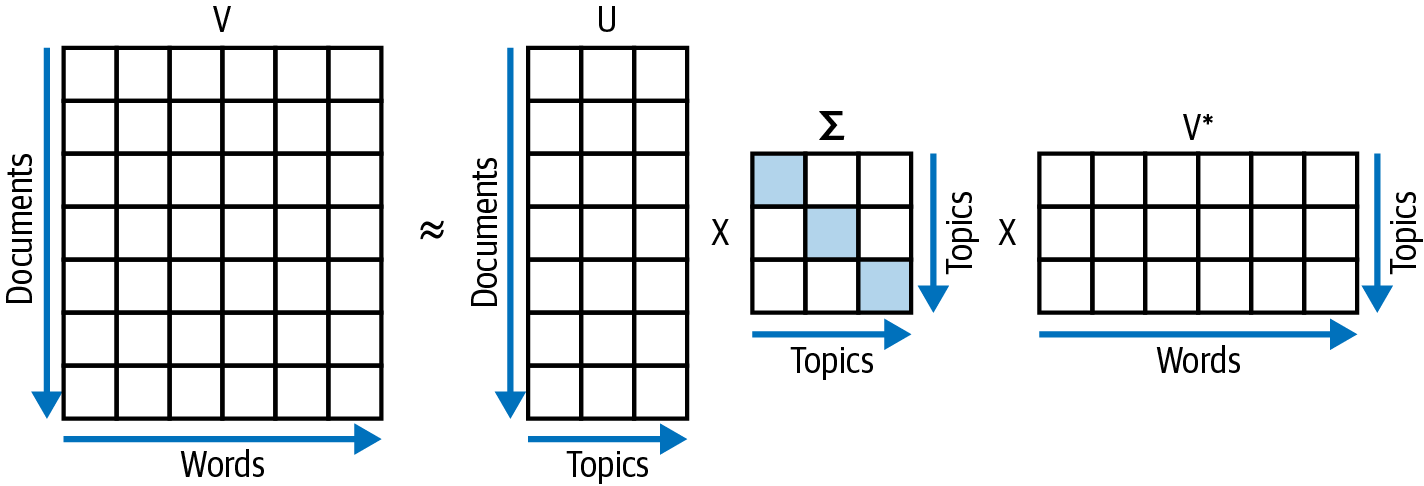
\includegraphics[width=0.70\textwidth]{Assets/svd}
    \caption{\gls{svd}: Source: \cite{blueprints}}
    \label{fig:svd}
\end{figure}

The nice thing about the \gls{svd} is that the quadratic Topics-Topics matrix (third matrix from left in Figure \ref{fig:svd}) on its diagonal contains the singular values which express the importance of each topic in a document.
A higher singular value indicates a topic that captures more of the variance (or information) in the corpus \cite{blueprints}.
From the most right Words-Topic matrix, the most important words per topic again can be extracted as described above (Section \ref{subsec:nmf}).

\subsection{\gls{lda}}\label{subsec:lda}
Latent Dirichlet Allocation (\gls{lda}), before the arrival of \glspl{llm}, had been the most prominent method for Topic Modelling \cite{blueprints}.
\gls{lda}, contrary to the previous methods above, is a probabilistic method that is based on the assumption that each Document contains a mix of a few different topics.
The method starts by randomly allocating words to each topic and also allocating topics to each document according to a Dirichlet distribution (\emph{Dirichlet prior}) \cite{blueprints}.
It then tries to re-create the words from the original document with stochastic sampling.
At the end of the optimization process, LDA also returns topics as a list of most frequent words as the \gls{nmf} and \gls{lda} methods do, but with a different distribution.

\section{Embedding-based Topic Modelling}\label{sec:topic_embedding_approaches}
As with most other fields in \gls{nlp}, the advent of \glspl{llm} also changed the way Topic Modelling can be approached today.
As the input data or features of traditional Topic Models are static words, they do to not take into account
the word's changing contextual meaning in different sentences, as already discussed in Section \ref{sec:word-embeddings}.
Thus, it is no wonder that today's best performing Topic Models are all embedding-based \cite{leaderboard-topic-models}.


\glspl{llm} can be used for Topic Modelling either with Pre-Trained or with \gls{gen-llm}s.

\subsection{Pre-Trained Topic Models}
Topic Modelling can be considered a classical text classification task and there are many pre-trained, publicly available models on HuggingFace \cite{huggingface} (see Figure \ref{fig:huggingface-topic-models}) or other platforms, even for multilingual text.

\begin{figure}[H]   %[h] puts picture right here. 't' stands for to, 'b' stands for bottom
    \centering
    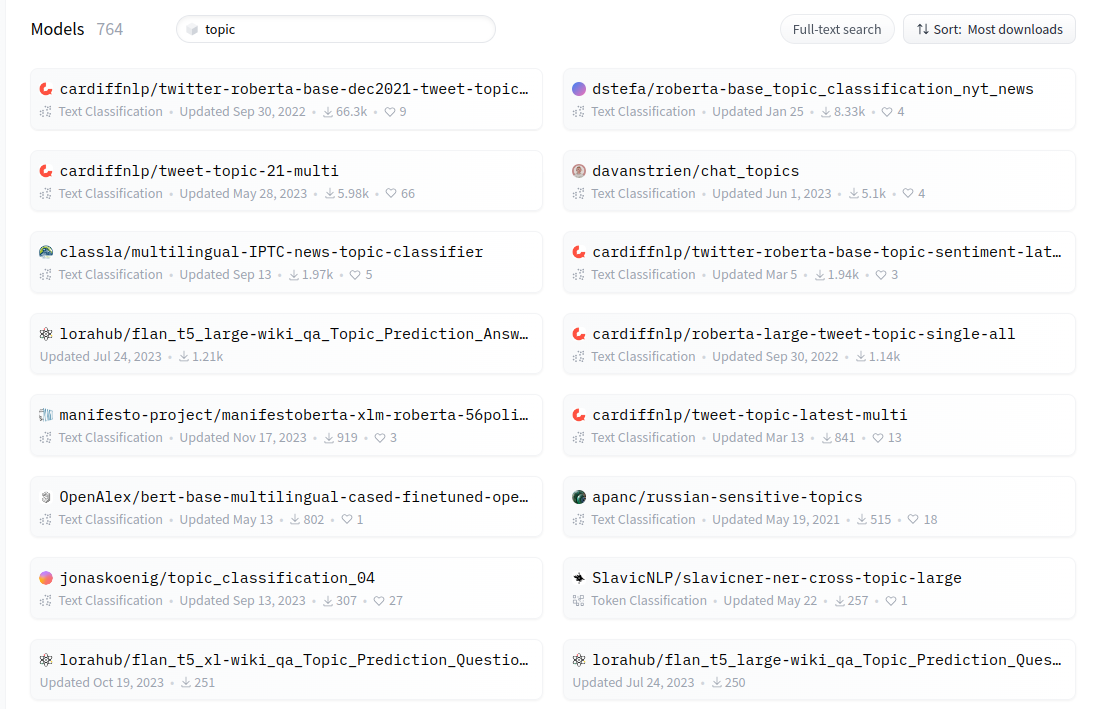
\includegraphics[width=0.85\textwidth]{Assets/huggingface-topic-models}
    \caption{Hugging Face Topic Models. Source: \cite{huggingface}}
    \label{fig:huggingface-topic-models}
\end{figure}

Unfortunately, the pre-trained Topic Models on Hugging Face \cite{huggingface} are either trained on labels that are very broadly categorized (see Figure \ref{fig:huggingface-topic-labels}) or very tightly confined to a narrow domain or language.

\begin{figure}[H]
\centering
\begin{minipage}{.35\linewidth}
  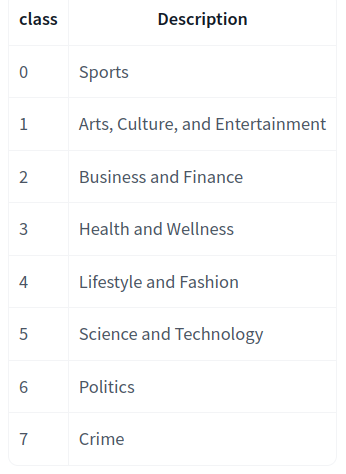
\includegraphics[width=\linewidth]{Assets/topic-classes-1}
  \label{img1}
\end{minipage}
\hspace{.05\linewidth}
\begin{minipage}{.55\linewidth}
  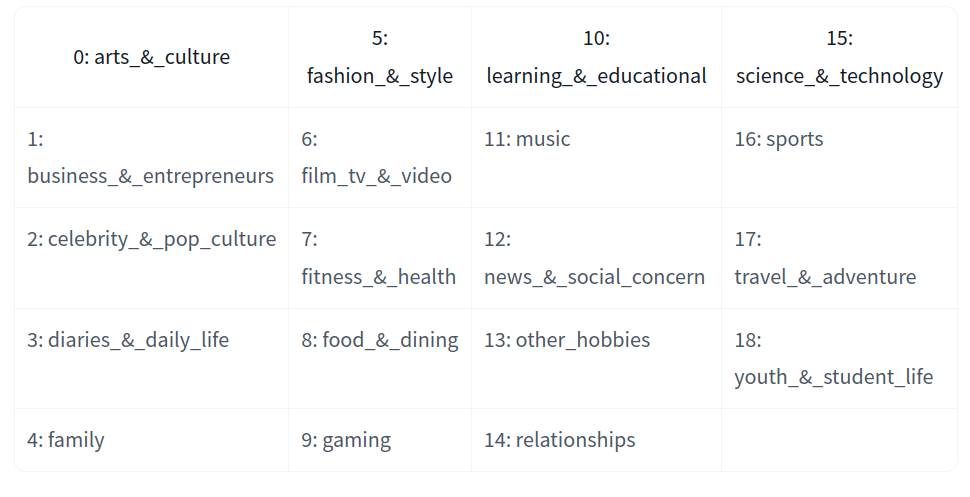
\includegraphics[width=\linewidth]{Assets/topic-classes-2}
  \label{img2}
\end{minipage}
    \captionof{figure}{Hugging Face Topic Models - Typical labels. Sources: \cite{topic-cardiffnlp}\cite{topic-stefanidis}}
    \label{fig:huggingface-topic-labels}
\end{figure}

After extensively researching the domains of these models, I conclude that none of them fits the corporate financial news domain and the given data very well.

It could be possible to fine-tune a model and I would expect the performance of such models to be quite good.
But fine-tuning would require to label and compile a lot of training samples which would go beyond the scope of this thesis.

\subsection{BERTopic}\label{subsec:bertopic}
Another kind of pre-trained model is BERTopic \cite{bertopic}.
BERTopic is similar to traditional models in that it returns a most-common-word list per topic for which the user must define a topic label manually.
But it differs from traditional models in that it does not use word vectors but Sentence Transformer (or SBERT) \cite{sentence-bert} embeddings.
BERTopic further uses dimension reduction and clustering techniques. \\
SBERT is a modification of the pre-trained \gls{BERT} model that uses siamese and triplet network structures to derive semantically meaningful sentence embeddings that can be compared using cosine-similarity.
This reduces the effort for finding the most similar pair of sentences significantly, while maintaining the accuracy from BERT \cite{sentence-bert}. \\


BERTopic \cite{bertopic} is a modular system in the sense that individual components can be substituted depending on the dataset and use case.
The modules and main steps to compose BERTopic \cite{bertopic} are:

\begin{enumerate}
    \item \textbf{Embeddings}: Choose and apply an embedding component, typically SBERT \cite{sentence-bert}
    \item \textbf{Dimension Reduction}: Choose and apply a dimension reduction method on the embeddings
    \item \textbf{Clustering}: Choose and apply a clustering algorithm on the dimension-reduced embeddings
    \item \textbf{Aggregate Text}: Aggregate the text of all documents within each cluster
    \item \textbf{Apply \gls{tfidf} Vectorization}:  Apply \gls{tfidf} vectorization to each of the per-Cluster-aggregated texts \footnote{In BERTopic, this is called class-based \gls{tfidf} or \emph{c-TF-IDF}}
    \item \textbf{Most Frequent Words}: Get the most frequent words for each cluster according to \gls{tfidf}
\end{enumerate}

This approach ensures that the distinction of Topic Clusters is made on the basis of contextual embeddings (Step 1).
But it also ensures, that the Topic that each Cluster represents, can also be presented as a collection of its most frequent words (Step 4 and 5).

BERTopic \cite{bertopic} can be downloaded and is pip-installable.
Most of the components in BERTopic are built with existing libraries such as Scikit-Learn.
I also wanted to compare it with traditional Topic modelling approaches, so I decided to implement it myself.
In this proprietary implementation not only word embeddings can be used, but also traditional word vectors such as those used in a classic Bag-of-Word (Sec.\ref{subsec:bag-of-words}) or \gls{tfidf} (Sec.\ref{subsec:tf-idf}) approach.\\

The modules for the self-implemented models can be found in the
\begin{center}
\emph{src/E\_topic\_model/traditional}
\end{center}
directory.
The model follows the modularity and architecture of BERTopic in that the steps to build the model are similar:

\begin{enumerate}
    \item \textbf{topic\_prepare}: If desired, preprocesses the text to reduce the dimension of the \gls{vocabulary} as described in Section \ref{subsec:techniques-to-reduce-vocabulary}.
    \item \textbf{topic\_vectorize}: Choose between \gls{tfidf} (Sec.\ref{subsec:tf-idf}), Bag-of-Word (Sec.\ref{subsec:bag-of-words}), One-Hot (Sec.\ref{subsec:one-hot-encoding}) vectorization or Sentence Transformers embeddings
    \item \textbf{topic\_dim\_reduce}: Choose between multiple dimension reduction methods such as PCA, \gls{nmf}, UMAP, etc.
    \item \textbf{topic\_cluster}: Choose between multiple cluster methods such as HDBSCAN, KMEANS, MEANSHIFT, etc.
    \item \textbf{topic\_model}: Run all of the above components and calculate Topics by presenting the most frequent words of each Cluster
    \item \textbf{topic\_visualize}: Reduce the dimension of the word vectors or embeddings to three and display the data and Clusters in a Plotly Scatter-3d-Graph.
\end{enumerate}

In the same directory, there are two Jupyter notebooks that can be used for model training and prediction:
\emph{topic\_model\_train.ipynb} and \emph{topic\_model\_test.ipynb}.

The Jupyter Notebook \emph{topic\_model\_train.ipynb} was used to extensively test different combinations of text processing approaches, vectorization methods and
cluster algorithms, but the results were disappointing.

\paragraph{Sentence Transformer Embeddings}
When using the Sentence Transformer embedding method as BERTopic does by default, the Cluster algorithms all had difficulties in separating the data points, not
only visually (see Figure \ref{fig:topic-embedd-cluster}), but also by separating semantically coherent words and sentences into different Clusters.

\begin{figure}[H]   %[h] puts picture right here. 't' stands for to, 'b' stands for bottom
    \centering
    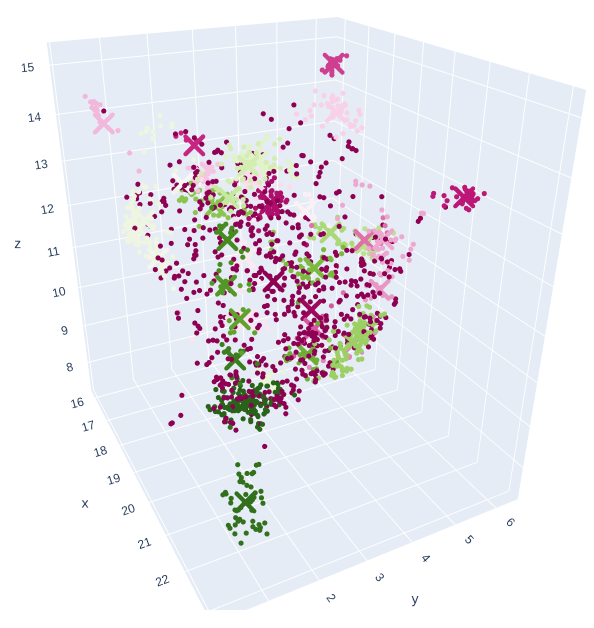
\includegraphics[width=0.50\textwidth]{Assets/topic-embedd-cluster}
    \caption{SBERT/Sentence Transformer embedding Cluster}
    \label{fig:topic-embedd-cluster}
\end{figure}

In Figure \ref{fig:topic-embedd-cluster}, UMAP was used to reduce the dimension to 20 and HDBSCAN was used to find clusters.
Although there are some clusters that are clearly separate from others, most of the clusters are within a close distance and the
separation of datapoints changes quickly with slightly different model parameters.
The same words appear in many clusters and manually looking at some individual sentences leads to the conclusion that sentences within clusters are not coherent.
The results were similar for other combinations of dimension reduction and clustering algorithms.

\paragraph{Word Vectors}
Looking at models were word vectors instead of embeddings were used, the performance of these models is not better:
\begin{figure}[H]   %[h] puts picture right here. 't' stands for to, 'b' stands for bottom
    \centering
    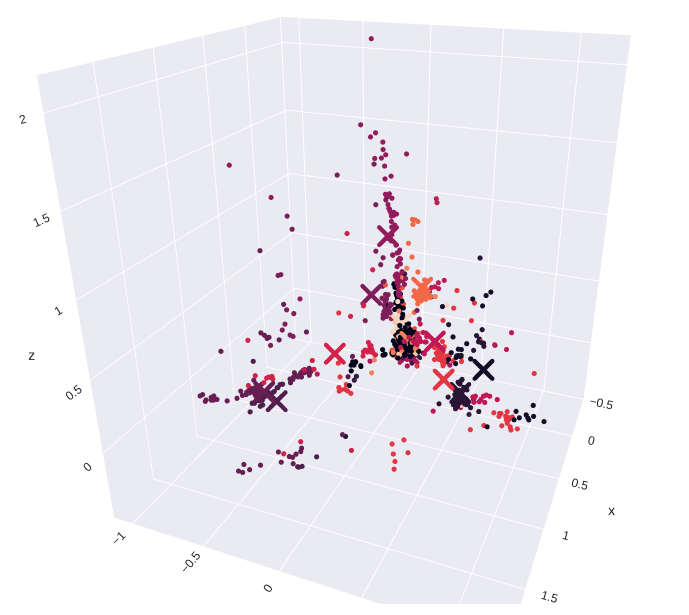
\includegraphics[width=0.50\textwidth]{Assets/topic-tfidf-cluster}
    \caption{TF-IDF Cluster}
    \label{fig:topic-tfidf-cluster}
\end{figure}

In Figure \ref{fig:topic-tfidf-cluster}, \gls{tfidf} was used for vectorization, PCA for dimension reduction and KMEANS for clustering.
The models suffer from the same shortcomings as the embedding based model above: same words appear in many clusters and sentences within clusters are not coherent.

\paragraph{Performance}
Although the financial news domain spreads across a wide range of topics, these topics are very nuanced and all have to do with company news.
I attribute the performance problems of the above methods to the fact that the differences between the individual sentences expressed
as distances in vector space are probably too small to extract meaningful clusters.

\section{Topic Modelling with \gls{gen-llm}s}\label{sec:topic-gen-llm}
Similar to creating a \gls{gen-llm} model for \gls{coref_resolution_definition}, the \gls{gen-llm} for Topic Modelling was also created with LangChain \cite{LangChain}.
As the problem of unresolvable dependency conflicts with existing Python libraries prevailed, the approach was again isolated with Docker.
The files for building the Docker container can be found in the
\begin{center}
\emph{/src/E\_topic\_model/img\_llm\_extract\_topics}
\end{center}
directory.

\paragraph{Data Model}
The \emph{data\_models.py} file in this directory contains the Python Enum \emph{TopicExplain} with the desired topic classes and a short description of each topic:

\begin{listing}[H]
    \captionof{listing}{Topic Model: Pre-Defined topics}
    \inputminted[
    firstline=9,
    lastline=29,
    firstnumber=9,
    fontsize=\tiny,
    ]{python}{/media/rainergo/PROJECTS/UASFRA-MS-Thesis/src/E_topic_model/img_llm_extract_topic/data_models.py}
    \label{code:llm-extract-topic-classes}
\end{listing}

There are 17 pre-defined topics formulated in German that were manually crafted by reading some of the article's sentences.
\emph{topic16} is dedicated to sentences that are incomplete and \emph{topic17} to all topics that are not covered by the previous 16 topics.\\

The process of defining topics could be facilitated by letting an \gls{llm} classify a set of sample sentences into an arbitrary number of topics, summarize each topic and express its overarching theme in a short sentence.
If manually crafted though, for a production use case, a more thorough semantic analysis of the article sentences and a re-assessment over the number of topics was also necessary.\\

The directory also contains a \emph{topics.py} file that provides sample sentences for each topic which are later used in the \gls{prompt} as few-shot examples.
Some of these few-shot examples are shown in Python-Code \ref{code:topic-examples}:

\begin{listing}[H]
    \captionof{listing}{Topic Model: Few Shot Examples}
    \inputminted[
    firstline=80,
    lastline=89,
    firstnumber=80,
    ]{python}{/media/rainergo/PROJECTS/UASFRA-MS-Thesis/src/E_topic_model/img_llm_extract_topic/topics.py}
    \label{code:topic-examples}
\end{listing}

As the few-shot examples often contain concrete company names, these company names therein were replaced by a \emph{Comp@Name@Placeholder} mask to avoid that the \gls{gen-llm} tries to match the company name of the sample sentence.\\

\paragraph{LangChain Code}
The LangChain code used in the Docker container is laid out in the \emph{topic\_langchain.py} file of the same directory, see Python-Code \ref{code:topic-langchain}:

\begin{listing}[H]
    \captionof{listing}{LangChain Topic Model}
    \inputminted[
    firstline=20,
    lastline=40,
    firstnumber=20,
    ]{python}{/media/rainergo/PROJECTS/UASFRA-MS-Thesis/src/E_topic_model/img_llm_extract_topic/topic_langchain.py}
    \label{code:topic-langchain}
\end{listing}
In line 26, the chain is built by \emph{piping} or connecting LangChain's \gls{prompt} component with the \gls{llm} component.
The \gls{prompt} contains the previously discussed few-shot \emph{examples} (line 27) compiled and organized by a Python function into an appropriate format.
It also contains the topics and their short descriptions (line 28) coming from the Python Enum \emph{TopicExplain} discussed above.\\

The sentences to be topic-classified are inserted into the \gls{prompt} (line 40) via an instance of a Python \emph{Frame} class (see Python-Code \ref{code:llm-extract-frame-class}) that inherits from Pydantic's BaseClass \cite{Pydantic}.
The same class in line 25 is also used in LangChain's \emph{ChatOpenAI} module function
\begin{center}
    \emph{llm.with\_structured\_output(schema=Frame)}
\end{center}
to force the \gls{llm} to return its response in the format of this class, as explained in Section \ref{par:coref-data-model}.

\begin{listing}[H]
    \captionof{listing}{Frame: A Pydantic BaseModel class}
    \inputminted[
    firstline=53,
    lastline=57,
    firstnumber=53,
    ]{python}{/media/rainergo/PROJECTS/UASFRA-MS-Thesis/src/E_topic_model/img_llm_extract_topic/data_models.py}
    \label{code:llm-extract-frame-class}
\end{listing}

\paragraph{Aggregation of Sentences}
The \emph{Frame} class, as the name implies, shall carry the data of a pandas DataFrame, namely the row \emph{indexes} of the DataFrame, the name of the column that contains the \emph{sentences} to be topic-classified and the \emph{topics} classes of those sentences to be returned by the \gls{gen-llm}.
The sentences to be classified are aggregated within a pandas DataFrame because the few-shot examples baked into the \gls{prompt} are rather long.
It would be very costly if the \gls{prompt} with its long few-shot examples would be sent for each sentence individually and separately.

\paragraph{The Token Limit Problem}
If there are many and long sentences to be topic-classified, the token limit that all \gls{gen-llm}s have imposed, will be reached.
To avoid that, the pandas DataFrame, later to be converted to a \emph{Frame} instance, first must be split into chunks.\\

This is what the function
\begin{center}
\emph{get\_topics\_from\_gen\_llm()} (Python-Code \ref{code:get-top-from-gen-llm})
\end{center}
in the \emph{main\_process.py} file will do.

\begin{listing}[H]
    \captionof{listing}{Frame: A Pydantic BaseModel class}
    \inputminted[
    firstline=124,
    lastline=157,
    firstnumber=124,
    ]{python}{/media/rainergo/PROJECTS/UASFRA-MS-Thesis/main_process.py}
    \label{code:get-top-from-gen-llm}
\end{listing}
It first chunks the passed DataFrame into a default size of 30 rows (line 130), converts it to a \emph{Frame} instance (line 131) and sends
the JSON-ized instance to the Docker container waiting for requests (line 133).
The LangChain model, as described above, in the Docker container forwards the Examples- and Topic-enhanced \gls{prompt} request to an OpenAI server and returns
the response from there, ideally in JSON-format (that complies with the \emph{Frame} class format), in line 140.

If the procedure succeeds, the topic classification of the \gls{gen-llm} for each DataFrame chunk first gets appended to a Python list that later will be used to create a new \emph{topics} column in the DataFrame.
If the procedure fails, it is tried once again and the request is resend.
If the procedure still fails, \emph{topic17} as the default spare class will be appended to the Python list in line 152.

The function returns the pandas DataFrame with an extra \emph{topics} column that contain one of the 17 Enum topics for each sentence.

\subsection{Comparing Pre-Trained vs. \gls{gen-llm} approach}
As outlined above, the cluster based methods such as the self-implemented BERTopic model, did not perform well on the Topic Modelling task.
In addition, they require to manually formulate a topic based on the most frequent words of a cluster.

The \gls{gen-llm} on the other side did perform well on the sentences I tested it with.
Most of the sentences were classified correctly.
For sentences that were expected to be classified differently, the actual and expected topic classes and examples were ambiguous and probably need some refinement.

I attribute the good performance of the \gls{gen-llm} to the power of a really large \gls{llm} (such as OpenAI's 4o model) that has the capacity to understand and distinguish even the most nuanced context.

I would expect a pre-trained \gls{llm}, such as those available on HuggingFace, to perform equally well after fine-tuning it with domain-specific topic labels and training data.

But as I did not go through the extensive process to compile and label such training data, in the project the \gls{gen-llm} was used for Topic Modelling.

\section{Information Extraction Pipeline}
After the Topic Modelling component has run, the \gls{gen-llm} has filled the pandas DataFrame column \emph{topics} in respect to each sentence in the column \emph{top\_sent}:
\begin{figure}[H]   %[h] puts picture right here. 't' stands for to, 'b' stands for bottom
    \centering
    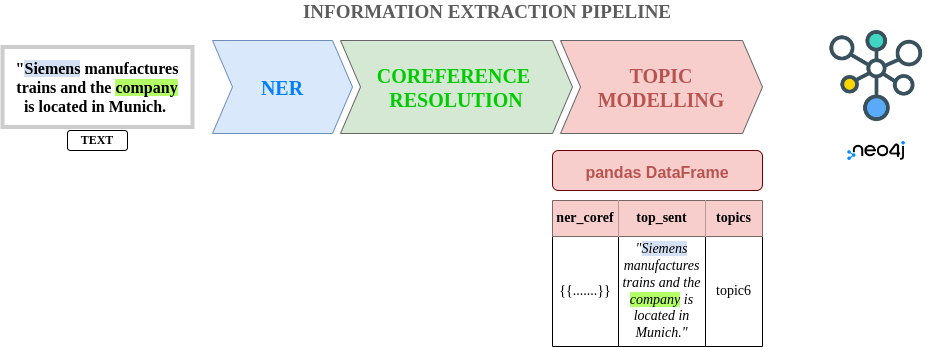
\includegraphics[width=0.90\textwidth]{Assets/pipelineTopic}
    \caption{DataFrame after Topic component}
    \label{fig:pipeTopic}
\end{figure}
In the example above, the DataFrame contains all the information coming from the \gls{ner} and \gls{coref_definition} components and one of the 17 possible topics for each sentence in which a company was found.


